
\begin{figure}
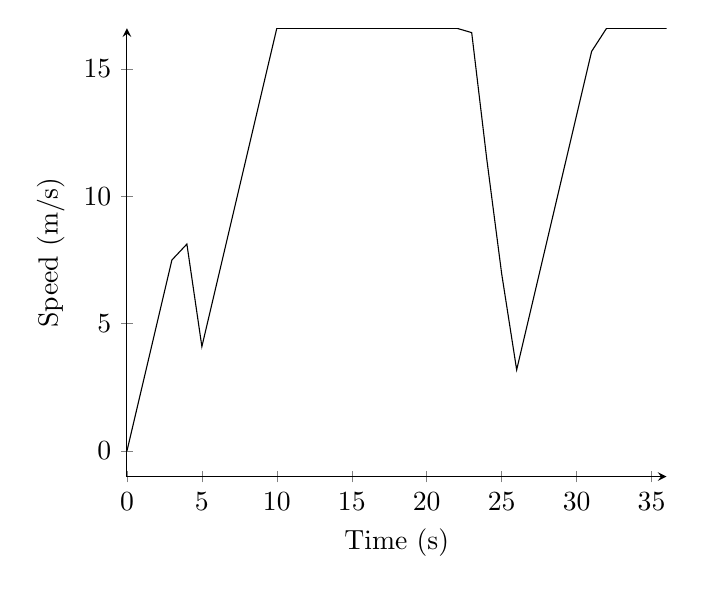
\begin{tikzpicture}
\begin{axis}[
legend style={anchor=west},
axis x line=bottom,
axis y line=left,
ymin=-1,
xlabel=Time (s),
ylabel=Speed (m/s),
]
\addplot[] coordinates {
(0, 0.0)
(1, 2.5)
(2, 5.0)
(3, 7.5)
(4, 8.12657070913)
(5, 4.10154203528)
(6, 6.60154203528)
(7, 9.10154203528)
(8, 11.6015420353)
(9, 14.1015420353)
(10, 16.6)
(11, 16.6)
(12, 16.6)
(13, 16.6)
(14, 16.6)
(15, 16.6)
(16, 16.6)
(17, 16.6)
(18, 16.6)
(19, 16.6)
(20, 16.6)
(21, 16.6)
(22, 16.6)
(23, 16.427407995)
(24, 11.488845972)
(25, 6.96123380583)
(26, 3.19014559729)
(27, 5.69014559729)
(28, 8.19014559729)
(29, 10.6901455973)
(30, 13.1901455973)
(31, 15.6901455973)
(32, 16.6)
(33, 16.6)
(34, 16.6)
(35, 16.6)
(36, 16.6)
};

\end{axis}
\end{tikzpicture}
\label{tik:speed:100:70}
\caption{100 percent diving with GSC on route $70$}
\end{figure}
